\documentclass[10pt,a4paper,fleqn]{article}
\usepackage[utf8]{inputenc}
\usepackage{amsmath}
\usepackage{amsfonts}
\usepackage{amssymb}
\usepackage[T1]{fontenc}
\usepackage{geometry}
\geometry{a4paper}
\usepackage[english]{babel}
\usepackage{dcolumn}
\usepackage{graphicx}
\usepackage{ntheorem}
\theoremseparator{:}
\newtheorem{theorem}{Hypothesis}
\usepackage{chngcntr}
\newcounter{pretheorem}
\counterwithin{theorem}{pretheorem}
\usepackage{caption}
\usepackage{textcomp}
\usepackage[export]{adjustbox}
\usepackage{float}
\usepackage{grffile}
\usepackage{listings}
\usepackage{fixltx2e}
\usepackage{verbatim}
\usepackage[backend=bibtex]{biblatex}
\usepackage[nottoc,numbib]{tocbibind}
\usepackage{setspace}
\usepackage{relsize}
\usepackage[final]{pdfpages}


\renewcommand\thetheorem{\arabic{pretheorem}\alph{theorem}}
\newcommand{\theoremgroup}{\refstepcounter{pretheorem}}

\renewcommand{\topfraction}{.85}
\renewcommand{\bottomfraction}{.7}
\renewcommand{\textfraction}{.15}
\renewcommand{\floatpagefraction}{.66}
\renewcommand{\dbltopfraction}{.66}
\renewcommand{\dblfloatpagefraction}{.66}
\setcounter{topnumber}{9}
\setcounter{bottomnumber}{9}
\setcounter{totalnumber}{20}
\setcounter{dbltopnumber}{9}


\doublespacing
\addbibresource{sample.bib}
\author{Chong Kim}





\begin{document}

\begin{titlepage}
\date{}
	\centering

	{\scshape\LARGE Final Installment \par}
	\vspace{1cm}
	{\scshape\Large Asthma Treatment Pattern Longitudinal Analysis \par}
	\vspace{1.5cm}

	\vspace{2cm}
	{\Large\itshape Chong Kim\par}
	\vfill
	supervised by\par
	Dr.~Matthew \textsc{Strand}
	\vfill


	{\large \today\par}

\begin{flushleft}
The Department of Clinical Pharmacy (DOCP) has provided funding for this educational project but has not conducted the
research or written this report. While the authors have worked on the best information available to them, neither
DOBB/DOCP nor the authors shall in any event be liable for any loss, damage or injury howsoever suffered directly or
indirectly in relation to the report or the research on which it is based.
\\~\\
Reference herein to trade names and proprietary products without stating that they are protected does not imply
that they may be regarded as unprotected and thus free for general use. No endorsement of named products is
intended nor is it any criticism implied of other alternative, but unnamed, products.
\end{flushleft}

\end{titlepage}

\newpage
\tableofcontents
\addcontentsline{toc}{section}{References}
\begin{appendix}
  \listoffigures
  \listoftables

\end{appendix}



\newpage 
\section{Changes and Additions}
\subsection{Data Management}
\textbf{Change:} Previously the time since diagnoses was a continuous measure that had counts of days. The new time variable, that allows for estimable standard errors, is measured in years not days. This allowed for the model to have stable standard errors that were estimable.\\
\textbf{Inspection:} Check whether or not the data sets created for sensitivity analysis (n=300, 1000, and 5000) had the appropriate number of unique patients within the data.


\subsection{Modeling}
\textbf{Addition 1:} Sensitivity analyses using 300, 1k and 5k results in different significance values for demographic variables. \\
\textbf{Addition 2:} Sensitivity analyses using multiple sample data sets of size 1k results in age significance robust to sampling.\\
\textbf{Addition 3:} 5k sample indicates significance in age, region, and cci along with time. Association between treatment steps and these variables seem to be strongly associated based on p-value (<0.0001).\\
\textbf{Addition 4:} Added clustering component (random intercept for subjects) in the hypotheses section. \\
\textbf{Final Data use:} Using the 5k data set for hypothesis 1 and hypothesis 2a. The objective function was not obtained using the 5k data for hypothesis 2b so using 1k data for hypothesis 2b. 


\section{Hypotheses}
\textbf{Hypothesis 1: We hypothesize that the likelihood of asthma treatment step will be different for different patient characteristics.}

\theoremgroup
\begin{theorem}
The likelihood of asthma treatment step (ordinal variable) will be different for different patient characteristics.
\end{theorem}


\noindent \textbf{Hypothesis 2: We hypothesize that the likelihood of asthma exacerbation event will be different for different treatment patterns.}

\theoremgroup
\begin{theorem}
The likelihood of asthma exacerbation event (yes/no) will be different for different treatment patterns.
\end{theorem}

\begin{theorem}
The likelihood of asthma exacerbation event (nominal variable) will be different for different treatment patterns.
\end{theorem}

\section{Statistical Methods}
\subsection{Hypothesis 1}
Various treatment step patterns will be associated with patient characteristics as described in the covariates section using multinomial regression methods that account for the longitudinal (correlated) data structure of the treatment step patterns. Specifically, the regression model will be built using a generalized linear mixed model with a cumulative logit link and with multinomial distribution. There will be minimal model selection as we are going to include all of the covariates mentioned in the covariates section. 

\subsubsection{Model 1: Model with All Covariates}
Model with all covariates(baseline age, gender, chronic comorbidity index, time, baseline cost, and treatment step). Results should indicate the relationship between the baseline characteristics of subjects and the outcome, asthma treatment step. Repeated measure \textbf{R\textsubscript{i}} side random effects are not supported for multinomial distribution. 
\begin{flalign}
logit(P(Y_{i}<j)) & = \theta_{j} - \beta_{1}base age_{i} -   \beta_{2}cci_{i}-  \beta_{3}time_{il}- \beta_{4}base cost_{i} - gender_{k} - b_{i0} \\\nonumber
 & i=1,..,n; j=1,...,J-1 \ where \ J = 6\ steps; k=1,2;l=1,...,r_{i}; \\\nonumber
 & \theta_{j} = Threshold \ variable; \ b \sim N(0,\sigma_{b}^{2}) \nonumber
\end{flalign}

\subsubsection{Model 2: Polynomial Trend}
Predictor variables(baseline age, gender, chronic comorbidity index, time, baseline cost). Results should indicate the relationship between the baseline characteristics of subjects and the outcome, asthma treatment step.
\begin{flalign}
logit(P(Y_{i}<j)) & = \theta_{j} - \beta_{1}base age_{i} -   \beta_{2}cci_{i}-  \beta_{3}time_{il}- \beta_{4}base cost_{i} - gender_{k}  - b_{i0}  \\\nonumber
 & i=1,..,n; j=1,...,J-1 \ where \ J = 6\ steps; k=1,2;l=1,...,r_{i}; \\\nonumber
 & \theta_{j} = Threshold \ variable; \ b \sim N(0,\sigma_{b}^{2}) \nonumber
\end{flalign}

\subsection{Hypothesis 2a}
Asthma exacerbation events will be associated primarily with the asthma treatment steps along with additional covariates of interest using multinomial regression methods that account for the longitudinal (correlated) data structure of the asthma exacerbation event (yes/no). Specifically, the regression model will be built using a generalized linear mixed model with a logit link and with binomial distribution.


\subsubsection{Model 1:Simple Model with all covariates}
Model with all covariates(baseline age, gender, chronic comorbidity index, time, baseline cost, and treatment step). Results should indicate the relationship between the baseline characteristics of subjects and the outcome, asthma exacerbation events. Repeated measure \textbf{R\textsubscript{i}} side random effects are not supported for multinomial distribution.
\begin{flalign}
\log(\dfrac{p}{1-p}) & = \beta_{0} + \beta_{1}base age_{i} +   \beta_{2}cci_{i}+ \beta_{3}base cost_{i} + \beta_{4}time_{ij}  + gender_{k}    \\\nonumber
& \beta_{5}TS_{ij} + \beta_{6}TS_{ij}*time_{ij}  + b_{i0}  \nonumber i=1,..,n;k=1,2;j=1,...,r_{i}; \\\nonumber
& b \sim N(0,\sigma_{b}^{2}) \nonumber
\end{flalign}


\subsubsection{Model 2: Modeling polynomial trend for time}
Model 2 + Polynomial variables for time. Results should indicate the relationship between the baseline characteristics of subjects and the outcome, asthma treatment step.
\begin{flalign}
\log(\dfrac{p}{1-p}) & = \beta_{0} + \beta_{1}base age_{i} +   \beta_{2}cci_{i} + \beta_{3}base cost_{i} + \beta_{4}time_{il}  + \beta_{5}time^{2}_{il} + \\\nonumber
& gender_{k} + \beta_{5}TS_{ij} + \beta_{6}TS_{ij}*time_{ij} + b_{i0}  \\\nonumber  & i=1,..,n;k=1,2;j=1,...,r_{i};\ b \sim N(0,\sigma_{b}^{2}) \nonumber \nonumber
\end{flalign}

\subsection{Hypothesis 2b}
Asthma exacerbation events will be associated primarily with the asthma treatment steps along with additional covariates of interest using multinomial regression methods that account for the longitudinal (correlated) data structure of the asthma exacerbation event (yes/no). Specifically, the regression model will be built using a generalized linear mixed model with a generalized logit link and with multinomial distribution.


\subsubsection{Model 1: Model with all covariates}
Predictor variables(baseline age, gender, chronic comorbidity index, time, baseline cost, and treatment step). Results should indicate the relationship between the baseline characteristics of subjects and the outcome, asthma treatment step.
\begin{flalign}
\log(\dfrac{p_{ijc}}{p_{ij1}}) & = \beta_{0} + \beta_{1}base age_{i} +   \beta_{2}cci_{i}+ \beta_{3}base cost_{i} + \beta_{4}time_{ij}  + gender_{k} \\\nonumber
& \beta_{5}TS_{ij} + \beta_{6}TS_{ij}*time_{ij} + b_{i0}  \ for \ c=2,3,..,5  \ i=`,..,n;k=1,2;j=1,...,r_{i}; \ b \sim N(0,\sigma_{b}^{2}) \nonumber \nonumber
\end{flalign}

\subsubsection{Model 2: Modeling polynomial trend for time}
Model 1 + Polynomial variables for time. Results should indicate the relationship between the baseline characteristics of subjects and the outcome, asthma treatment step.
\begin{flalign}
\log(\dfrac{p_{ijc}}{p_{ij1}}) & = \beta_{0} + \beta_{1}base age_{i} +   \beta_{2}cci_{i} + \beta_{3}base cost_{i} + \beta_{4}time_{il}  + \beta_{5}time^{2}_{il} + \\\nonumber
& gender_{k} + \beta_{5}TS_{ij} + \beta_{6}TS_{ij}*time_{ij} + b_{i0} \\\nonumber
 & \ for \ c=2,3,..,5; \ i=`,..,n;k=1,2;l=1,...,r_{i}; b \sim N(0,\sigma_{b}^{2}) \nonumber
\end{flalign}

\section{New Results from Changes}
\subsection{Hypothesis 1}
\subsubsection{Final Output for Hypothesis 1}
\begin{figure}[!ht]
\label{h1f}
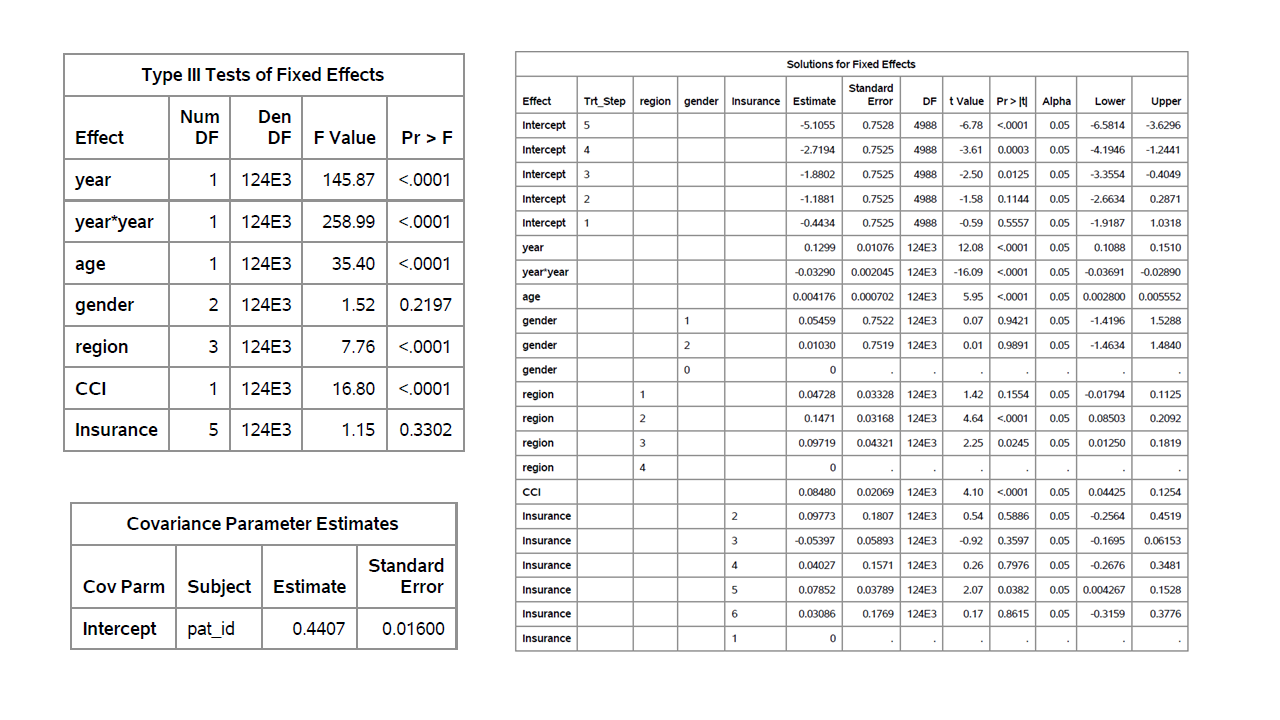
\includegraphics[width=\textwidth,height=\textheight,keepaspectratio]{C:/Users/ck/Dropbox/Academic Coursework/FS2016/Longitudinal/Project/Report/Model/11.29.2016/h15k.png}
\end{figure}
\newpage

\subsection{Hypothesis 2a}
\subsubsection{Final Output for Hypothesis 2a}
\begin{figure}[!ht]
\label{h2af}
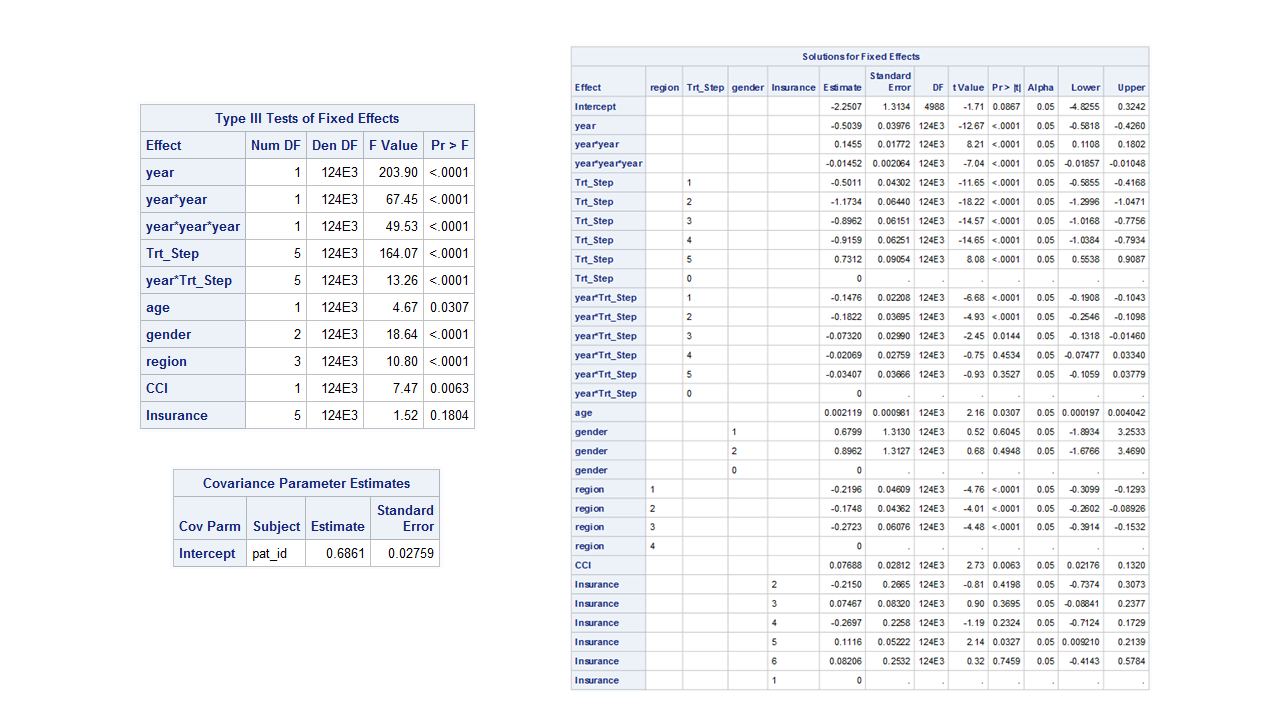
\includegraphics[width=\textwidth,height=\textheight,keepaspectratio]{C:/Users/ck/Dropbox/Academic Coursework/FS2016/Longitudinal/Project/Report/Model/11.29.2016/h2a5k.png}
\end{figure}
\newpage

\subsection{Hypothesis 2b}
\subsubsection{Final Output for Hypothesis 2b}
\begin{figure}[!ht]
\label{h2bf}
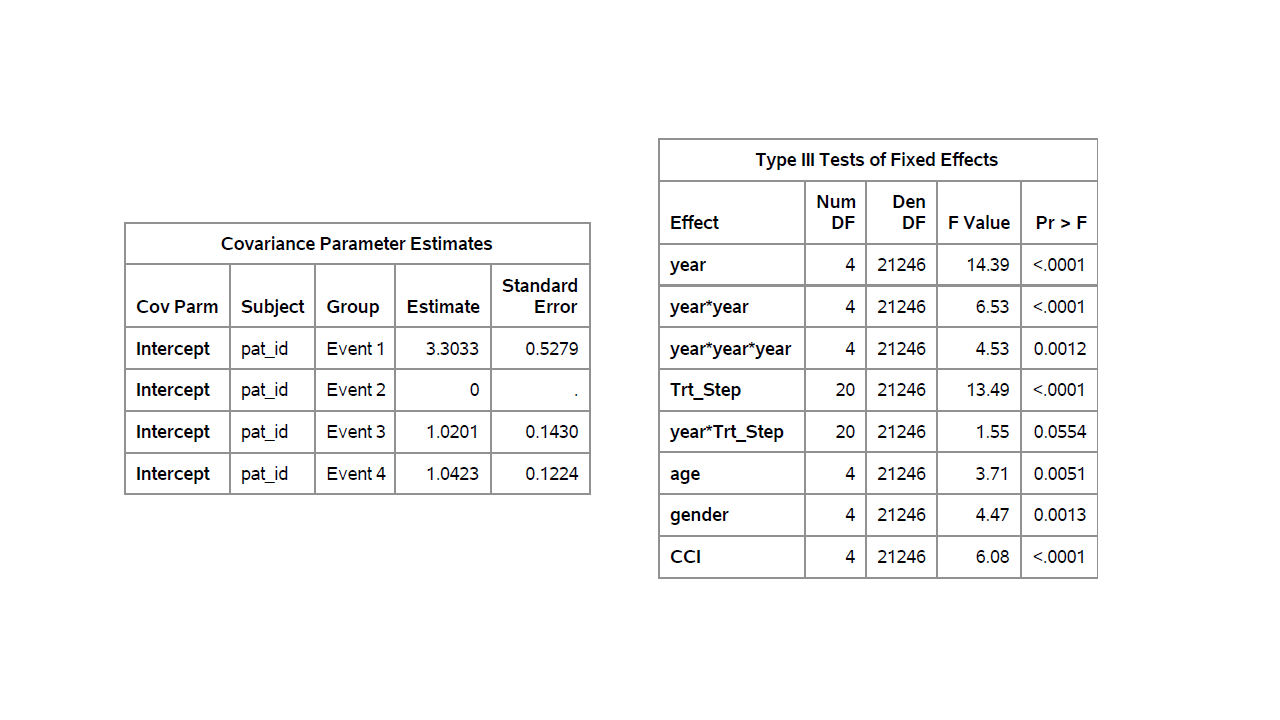
\includegraphics[width=\textwidth,height=\textheight,keepaspectratio]{C:/Users/ck/Dropbox/Academic Coursework/FS2016/Longitudinal/Project/Report/Model/11.29.2016/h2b1k.png}
\end{figure}

\newpage	
\section{Initial Descriptives}

\begin{table}[ht]
\centering
\resizebox{\columnwidth}{!}{%
\begin{tabular}{rllllllll}
\\[-1.8ex]\hline 
\hline \\[-1.8ex] 
 & \multicolumn{1}{c}{\textit{Baseline Treatment Steps}} \\ 
\cline{2-2} 
  \hline
 & 0 & 1 & 2 & 3 & 4 & 5 & p & test \\ 
  \hline
n & 781 & 112 & 39 & 38 & 26 & 4 &  &  \\ 
  age (mean (sd)) & 31.42 (17.95) & 28.00 (18.32) & 22.26 (16.32) & 29.89 (17.87) & 33.19 (18.94) & 42.00 (19.13) & 0.013 &  \\ 
  pat\_region (\%) &  &  &  &  &  &  & 0.206 &  \\ 
     E & 219 (28.0) & 25 (22.3) & 6 (15.4) & 10 (26.3) & 9 (34.6) & 2 (50.0) &  &  \\ 
     MW & 254 (32.5) & 40 (35.7) & 13 (33.3) & 15 (39.5) & 9 (34.6) & 1 (25.0) &  &  \\ 
     S & 229 (29.3) & 28 (25.0) & 15 (38.5) & 5 (13.2) & 5 (19.2) & 1 (25.0) &  &  \\ 
     W & 79 (10.1) & 19 (17.0) & 5 (12.8) & 8 (21.1) & 3 (11.5) & 0 (0.0) &  &  \\ 
  Insurance (\%) &  &  &  &  &  &  & 0.191 &  \\ 
     1 & 665 (85.1) & 90 (80.4) & 34 (87.2) & 29 (76.3) & 24 (92.3) & 3 (75.0) &  &  \\ 
     2 & 3 (0.4) & 1 (0.9) & 0 (0.0) & 1 (2.6) & 1 (3.8) & 0 (0.0) &  &  \\ 
     3 & 20 (2.6) & 8 (7.1) & 2 (5.1) & 1 (2.6) & 0 (0.0) & 1 (25.0) &  &  \\ 
     4 & 3 (0.4) & 1 (0.9) & 0 (0.0) & 1 (2.6) & 0 (0.0) & 0 (0.0) &  &  \\ 
     5 & 86 (11.0) & 11 (9.8) & 3 (7.7) & 6 (15.8) & 1 (3.8) & 0 (0.0) &  &  \\ 
     6 & 4 (0.5) & 1 (0.9) & 0 (0.0) & 0 (0.0) & 0 (0.0) & 0 (0.0) &  &  \\ 
  baseline\_cost (mean (sd)) & 2361.08 (7009.85) & 1506.44 (2521.98) & 1142.77 (1332.55) & 886.63 (1378.18) & 1734.34 (3036.80) & 1940.89 (504.53) & 0.455 &  \\ 
  CCI (mean (sd)) & 0.30 (0.62) & 0.18 (0.71) & 0.18 (0.56) & 0.05 (0.23) & 0.19 (0.49) & 0.25 (0.50) & 0.074 &  \\ 
   \hline
\end{tabular}%
}
\end{table}
\clearpage


\section{Graphical Visualization}
\begin{figure}[!htbp]
\caption{Correlation Matrix of Continuous Variables}
\label{fig1}
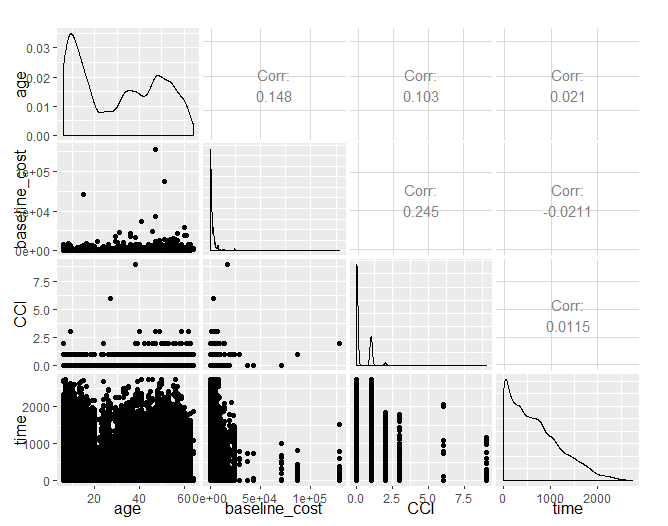
\includegraphics[scale=0.90]{C:/Users/ck/Dropbox/Academic Coursework/FS2016/Longitudinal/Project/Report/correlationmatrix.png}
\end{figure}
\newpage
\begin{figure}[!htbp]
\caption{Histogram of Continuous Variables by Event as Binary}
\label{fig2}
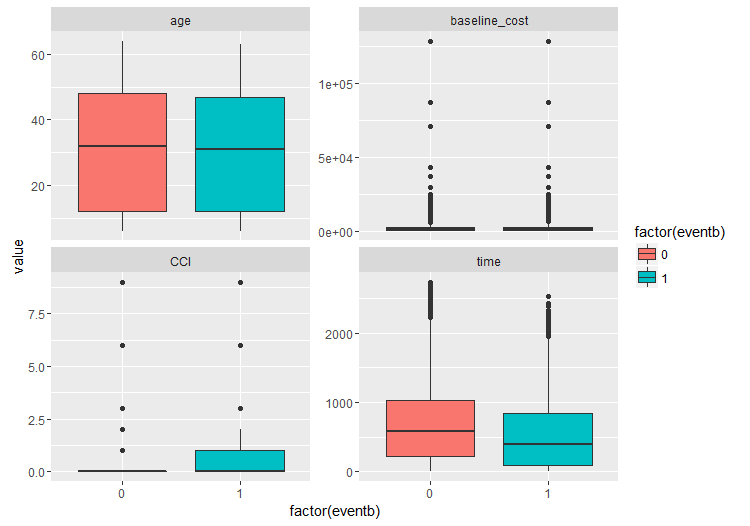
\includegraphics[scale=0.90]{C:/Users/ck/Dropbox/Academic Coursework/FS2016/Longitudinal/Project/Report/histogram.png}
\end{figure}
\newpage
\begin{figure}[!htbp]
\caption{Bubble Diagram of Treatment Step by Event as Binary}
\label{fig3}
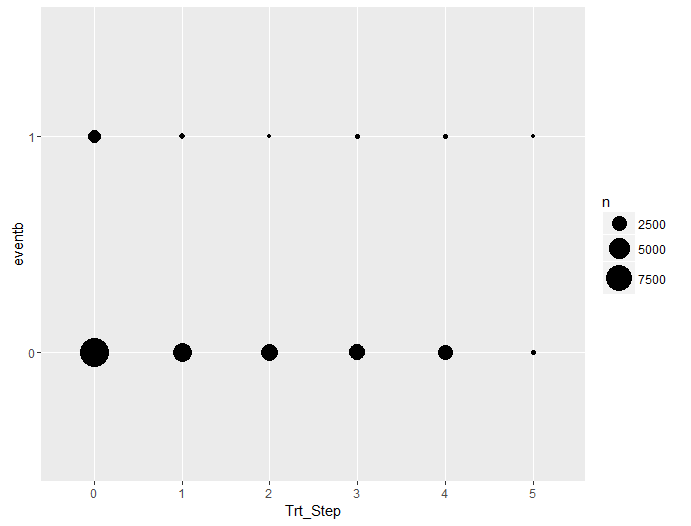
\includegraphics[scale=0.90]{C:/Users/ck/Dropbox/Academic Coursework/FS2016/Longitudinal/Project/Report/bubble.png}
\end{figure}
\newpage
\begin{figure}[!htbp]
\caption{Probability of Event by Time}
\label{fig4}
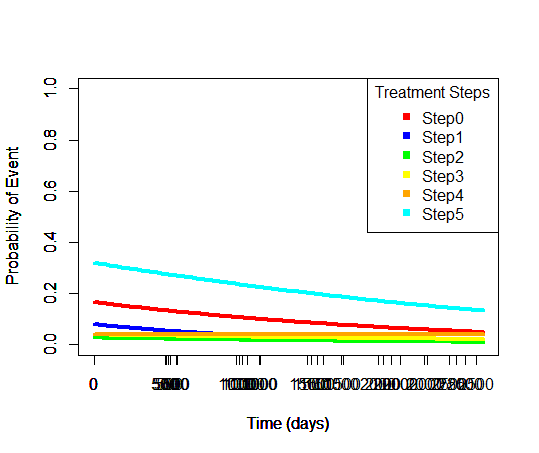
\includegraphics[scale=0.90]{C:/Users/ck/Dropbox/Academic Coursework/FS2016/Longitudinal/Project/Report/initialplot.png}
\end{figure}

\newpage


\section{Appendix}
\subsection{Description of Data}
There are currently 3 data sets.
\begin{itemize}
  \item Patient characteristic file
  \item Exposure file
  \item Outcome file
\end{itemize}
\textbf{Study period}: January 2006 \~ December 2013\\~\\
\textbf{Population:} All patients with asthma within most recent 10\% random sample database housed by CePOR\\~\\
\textbf{Patient entry criteria:}
\begin{enumerate}
  \item evidence of asthma at least two recorded diagnosis for asthma (icd\- 9:493.xx) within 1 year.
  \item having at least 24 months continuous eligibility after index date (follow-up period) and at least 6 months continuous eligibility before index date (pre\- period) environment.
  \item Age 6\- 64 at index.
\end{enumerate}
\textbf{Patient exclusion criteria:}
\begin{enumerate}
  \item diagnosed with cystic fibrosis  (ICD\- 9; 277.0x) or chronic obstructive pulmonary diseases (491.xx, 492.xx, 494.xx and 496.xx) or respiratory tract cancer (160.xx \- 164.xx or 231.xx) or bronchopulmonary dysplasia (770.7x) or respiratory distress syndrome (769.xx).
  \item one of the following diagnoses: Addison disease (255.4x), glomerulonephritis (580.xx to 582.xx), multiple sclerosis (340.xx), polymyositis/dermatomyositis (710.3x, 710.4x), rheumatoid arthritis (714.xx), scleroderma (710.1x), Sjogren disease (710.2x ), systemic lupus erythematosus (710.0x), uveitis (360.11, 363.20 364.3x ), vitiligo (709.01), Wegener granulomatosis (446.4x), Primary systemic vasculitis (447.6x), Crohn?s disease (555.0x to 555.2x, 555.9x), Ulcerative colitis (556.0x to 556.6x, 556.8x, or 556.9x), Chronic eosinophilic pneumonia (518.3x), Idiopathic pulmonary fibrosis (516.3x or 515.xx), minimal change disease (581.3x), autoimmune hepatitis (571.42), Myasthenia Gravis (358.0x), Muscular dystrophy (359.0x, 359.1x, or 359.21), Still?s disease (714.2x), Churg Strauss syndrome (446.4x), Polymyalgia rheumatica (725.xx)
\end{enumerate}
\textbf{Index date:} The first date of asthma diagnosis with 6 months eligibility before the index date (NOTE: asthma diagnosis can occur prior to the index date, however, these diagnoses would not have 6 months eligibility prior to the dates.) \\~\\

\subsection{Variables}
\textbf{Outcomes:}
The primary outcome of interest is a nominal variable that includes:
\begin{enumerate}
  \item No event.
  \item Asthma-related hospitalization.
  \item Asthma-related emergency department visit.
  \item Asthma-related outpatient exacerbation.
  \item Outpatient visit for lower respiratory tract infection treated with antibiotics. 
\end{enumerate}

(See codes and definition in excel)
For patients who have at least one event, we would like to have data on type of event in numeric format and number of days after the index date in numeric format. For those patients with at least one event, only the event category that are observed need to be included i.e. patients who have hospitalization and outpatient exacerbation would only have event 1 and 3 included in the outcome file.
For patient who do NOT have any events during the follow-up time, we would like to include them and have event = 0 and date = missing. 


\textbf{Exposure Variable:}
The primary exposure variable is treatment steps which is an ordinal variable characterized as:
\begin{figure}[!htbp]
\caption{}
\label{}
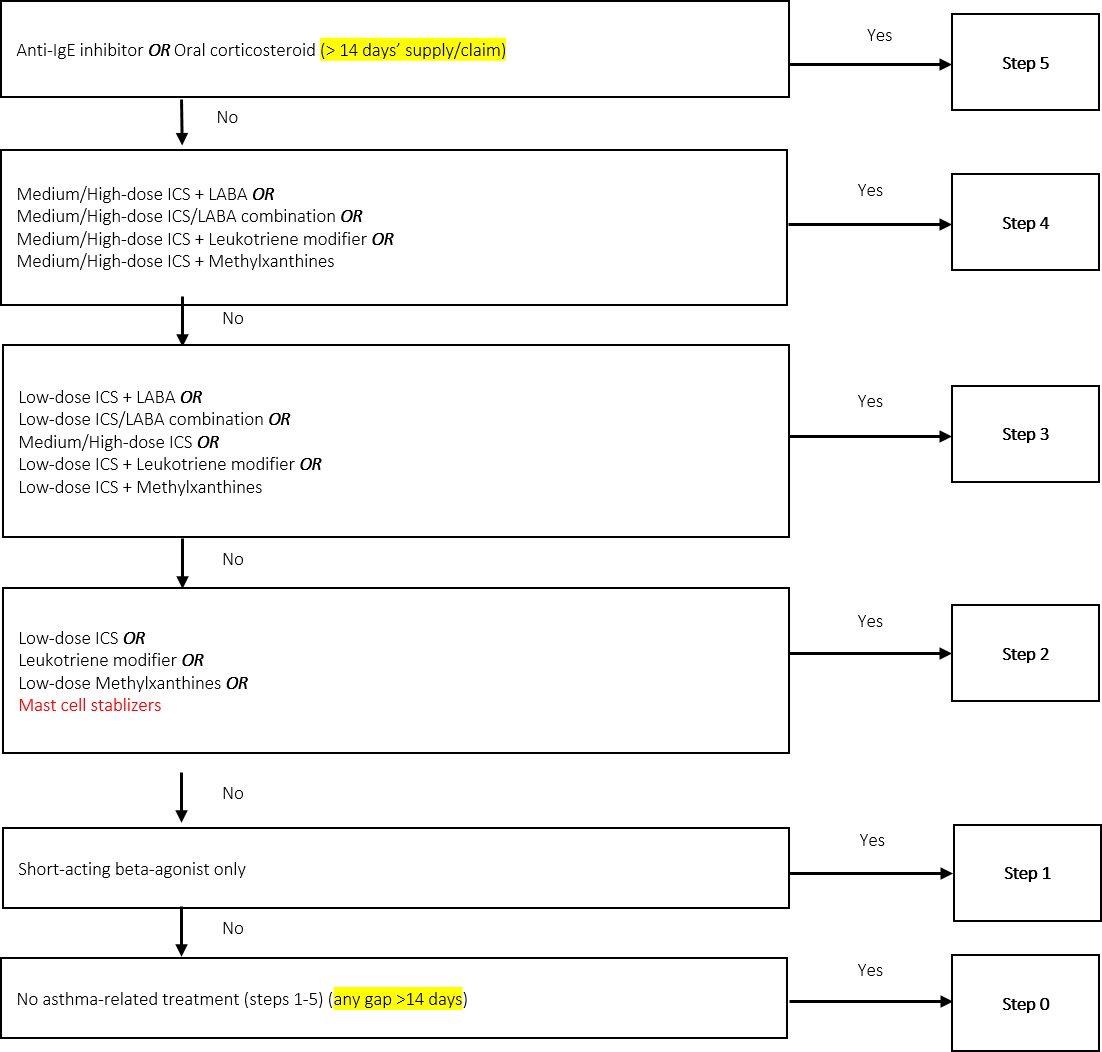
\includegraphics[scale=0.90]{C:/Users/ck/Dropbox/Academic Coursework/FS2016/Longitudinal/Project/Report/trt_step.png}
\end{figure}



\end{document}